\documentclass[a4paper]{article}    % define document layout
%\documentclass[draft]{article}     % use draft option in packages
%-----------------------------
% preamble
%-----------------------------
\usepackage[sumlimits,]{amsmath}    % math equations and formulas
\usepackage[utf8]{inputenc}         % use UTF-8 encoding
\usepackage[english]{babel}         % use English language
\usepackage{graphicx}              % insert images
%\usepackage[draft]{graphicx}        % do not render figures
\usepackage{subcaption}             % multiple images in one figure
\usepackage{hyperref}               % hyperlinks
\usepackage{float}                  % floating objects (figures, tables)
\usepackage{geometry}               % page size and margins
\geometry{a4paper, margin=1in}      % margins
\usepackage{ragged2e}               % text alignment
\usepackage[table]{xcolor}          % change cell color in tables
%\usepackage{multirow}               % merge rows in table
%\usepackage[thinc]{esdiff}          % macros for derivatives

% MATLAB code
\usepackage{listings}
\usepackage{color} %red, green, blue, yellow, cyan, magenta, black, white
\usepackage{xcolor}

\graphicspath{                      % path for figures
    {../figures/} 
}

\definecolor{codegreen}{rgb}{0,0.6,0}
\definecolor{codegray}{rgb}{0.5,0.5,0.5}
\definecolor{codepurple}{rgb}{0.58,0,0.82}
\definecolor{backcolour}{rgb}{0.95,0.95,0.92}

\lstdefinestyle{mystyle}{
    backgroundcolor=\color{backcolour},   
    commentstyle=\color{codegreen},
    keywordstyle=\color{magenta},
    numberstyle=\tiny\color{codegray},
    stringstyle=\color{codepurple},
    basicstyle=\ttfamily\footnotesize,
    breakatwhitespace=false,         
    breaklines=true,                 
    captionpos=b,                    
    keepspaces=true,                 
    numbers=left,                    
    numbersep=5pt,                  
    showspaces=false,                
    showstringspaces=false,
    showtabs=false,                  
    tabsize=2
}
\lstset{style=mystyle}

%-----------------------------
% body
%-----------------------------
\begin{document}

\begin{figure}
    \centering
    % UNICAMP logo
    \begin{subfigure}{0.45\textwidth}
        \centering
        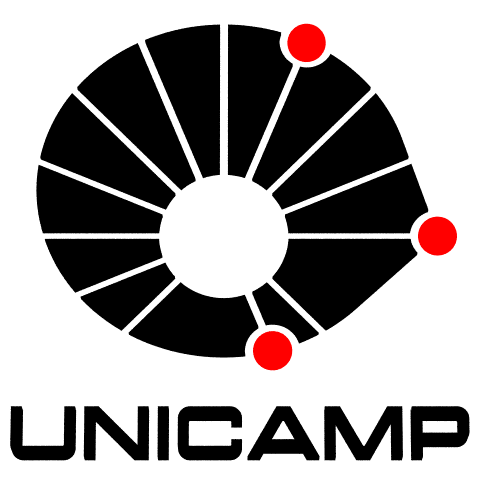
\includegraphics[width=1.5cm]{unicamp}
%        \label{fig:unicamp}
    \end{subfigure}
    \hfill
    % FEEC logo
    \begin{subfigure}{0.45\textwidth}
        \centering
        
\includegraphics[width=1.5cm]{feec}
%        \label{fig:feec}
    \end{subfigure}
\end{figure}

\title{
    \vspace{5cm}
    IA353A - Neural Networks\\
    EC2
    \vspace{1cm}
}
\author{
    Rafael Claro Ito\\
    (R.A.: 118430)
    \vspace{11cm}
}
%R.A.: 118430
%ito.rafael@gmail.com
\date{August 2020}
\maketitle
\newpage

\setcounter{section}{7}
%=================================================
\section*{Question 7}
%=================================================

%------------------------
\subsection{Transferência negativa}
%------------------------

%------------------------
\subsection{Camadas compartilhadas}
%------------------------

%------------------------
\subsection{MALSAR}
%------------------------

\newpage
%=================================================
\section*{Question 8}
%=================================================



\newpage
\setcounter{section}{9}
\setcounter{subsection}{0}
%=================================================
\section*{Question 9}
%=================================================

%------------------------
\subsection{Principais seções do padrão de documentação}
%------------------------

%------------------------
\subsection{Artigos com propósitos similares}
%------------------------

%------------------------
\subsubsection*{Artigo 1}
%------------------------

%------------------------
\subsubsection*{Artigo 2}
%------------------------

\newpage
\setcounter{section}{10}
\setcounter{subsection}{0}
%=================================================
\section*{Question 10}
%=================================================

%------------------------
\subsection{EfficientNet}
%------------------------

%------------------------
\subsection{FixEfficientNet}
%------------------------

%=================================================

\end{document}
